\subsection{Subpaso 1-A: Iniciar estadísticas por profesor}
	En la configuración de las estadísticas se tiene que seleccionar el 
	inciso \textbf{Por profesor} y el profesor que desea analizar. 
		
	\begin{figure}[hbtp]

	
\includegraphics[scale=0.5]{images/Interfaz/IUGS15_configuracionMes.PNG}
	\caption{Configuración por profesor }
	\end{figure}
	A continuación se aprieta el botón \textbf{Consultar Profesor}
	 
\subsection{Subpaso 1-B: Muestra de Estadísticas}
	Se mostrará la siguiente interfaz con las siguientes estadísticas:

	\begin{figure}[hbtp]
		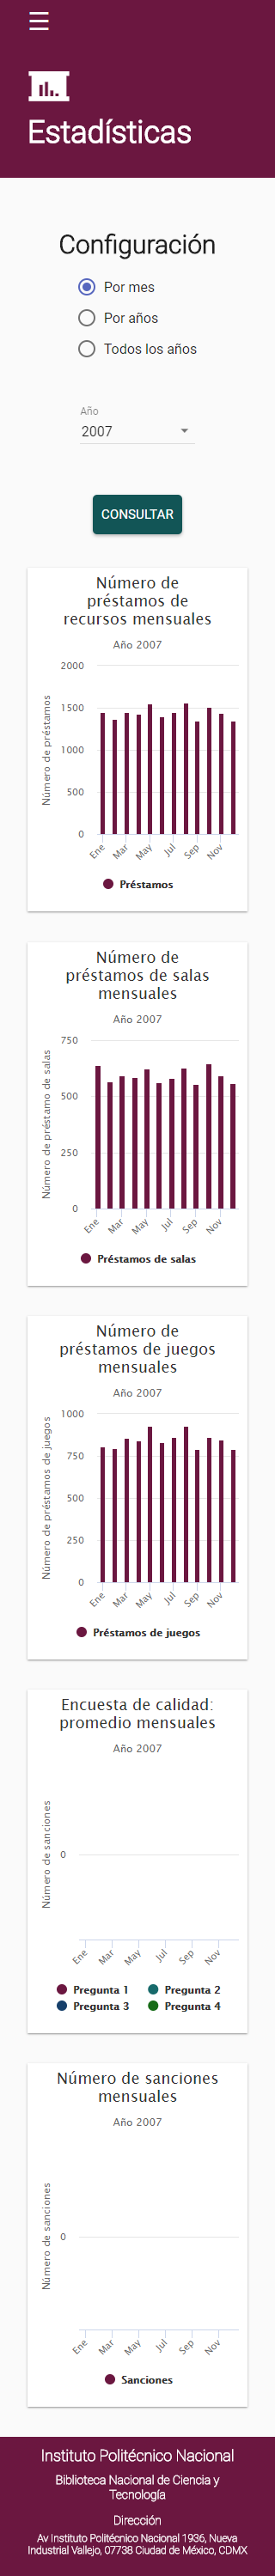
\includegraphics[scale=0.5]{images/Interfaz/IUGS15_estadisticasMes.PNG}
		\caption{Pagina general de Estadísticas por Profesor}
	\end{figure}	
	
\begin{itemize}
	\item  La información respectiva del profesor evaluado es la siguiente:
	\begin{enumerate}
		
		\item Nombre
		\item Edad
		\item Email
		\item País
		\item Institución 
		\item Área 
		\item Nivel
		
		
	\end{enumerate}
	\item Promedio de dificultad del cuestionario según el profesor.
	
	\item Una gráfica de barras la cual representa la dificultad por pregunta 
	con la	escala de 0 a 10.
	
\end{itemize}
\subsection{Subpaso 1-C: Muestra de Opinión por cada pregunta}
Se mostrarán las opiniones de cada de una de las preguntas del cuestionario.
\begin{figure}[hbtp]

	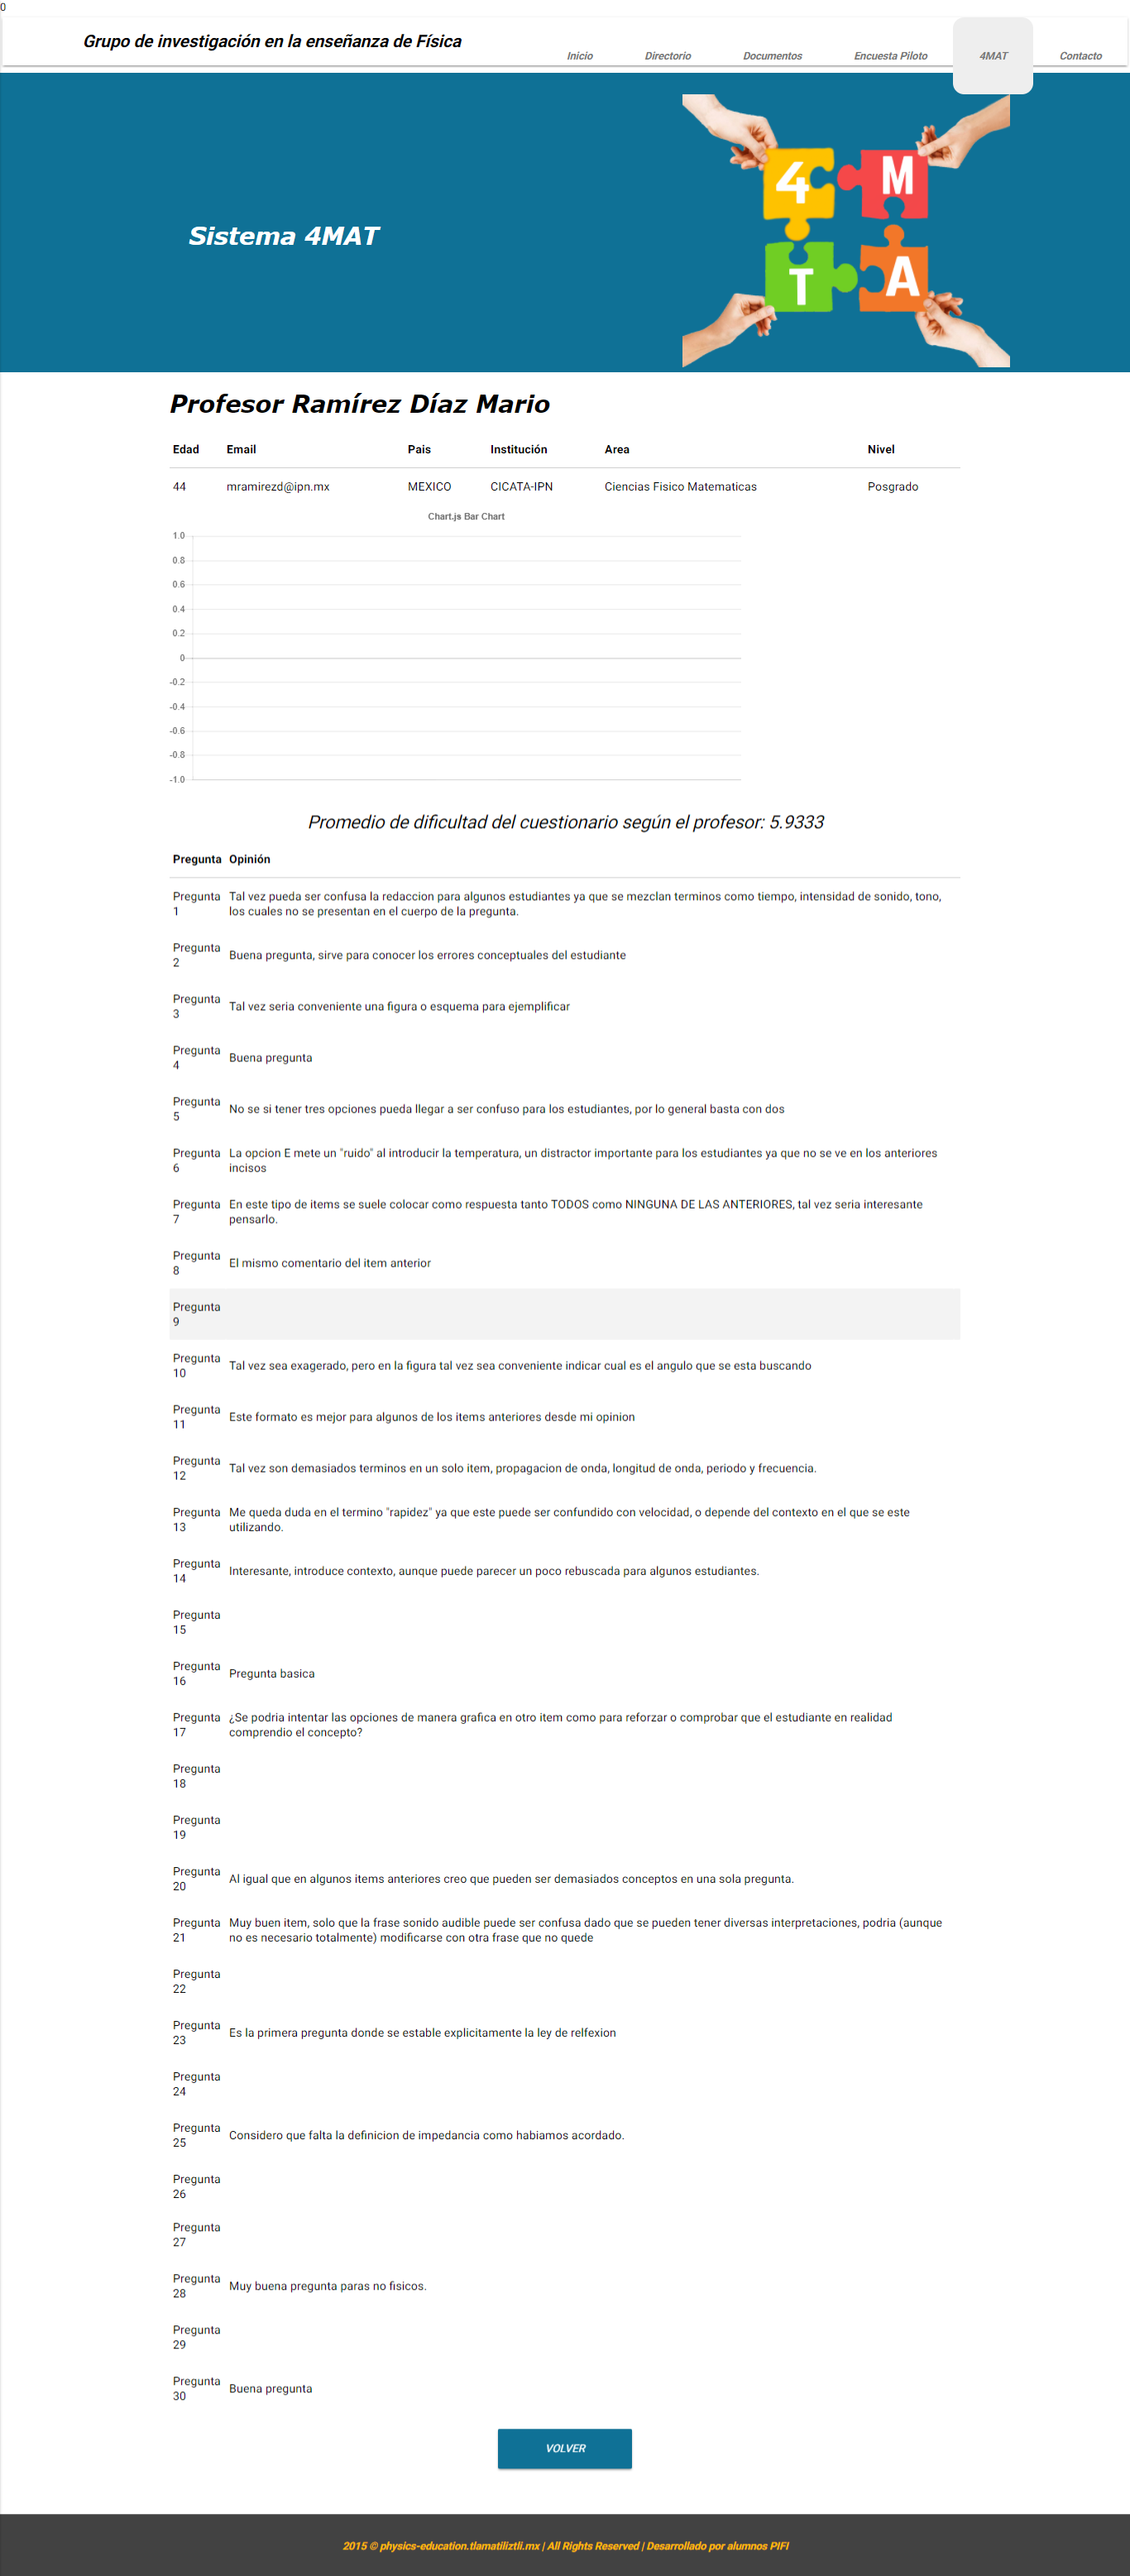
\includegraphics[scale=0.3]{images/Interfaz/IUGS15_opinionPregunta.PNG}
	\caption{Opinión por cada pregunta }
	\end{figure}